\documentclass[12pt, a4paper]{scrreprt}

%% Language and font encodings
\usepackage[ngerman]{babel}
\usepackage[utf8]{inputenc}
\usepackage[T1]{fontenc}
\usepackage{helvet}
\renewcommand{\familydefault}{\sfdefault}
\usepackage{bibgerm}

%% Sets page size and margins
\usepackage[a4paper,top=2.5cm,bottom=2cm,left=2cm,right=2cm]{geometry}

%% Useful packages
\usepackage{amsmath}
\usepackage{graphicx}
\usepackage[colorinlistoftodos]{todonotes}
\usepackage[colorlinks=true, allcolors=blue]{hyperref}

\setlength{\parindent}{0em}
\setlength{\parskip}{1em}

\usepackage{scrlayer-scrpage}
\KOMAoptions{
  headwidth=\textwidth+30pt:-15pt,
  headsepline=.2pt
}
%\clearpairofpagestyles
\ihead{Mr. Trash Design Dokument}
\chead{TU Wien, MSE}
\ohead{Hurbean, Schweiger [Gruppe 06]}
\renewcommand\chapterpagestyle{scrheadings}


\title{Mr. Trash}
\subtitle{App zur effizienten Müllentsorgung}
\author{
    Hurbean, Alexander\\
    \texttt{e1625747}
    \and
    Schweiger, Phillipp\\
    \texttt{e01634254}}
\titlehead{\centering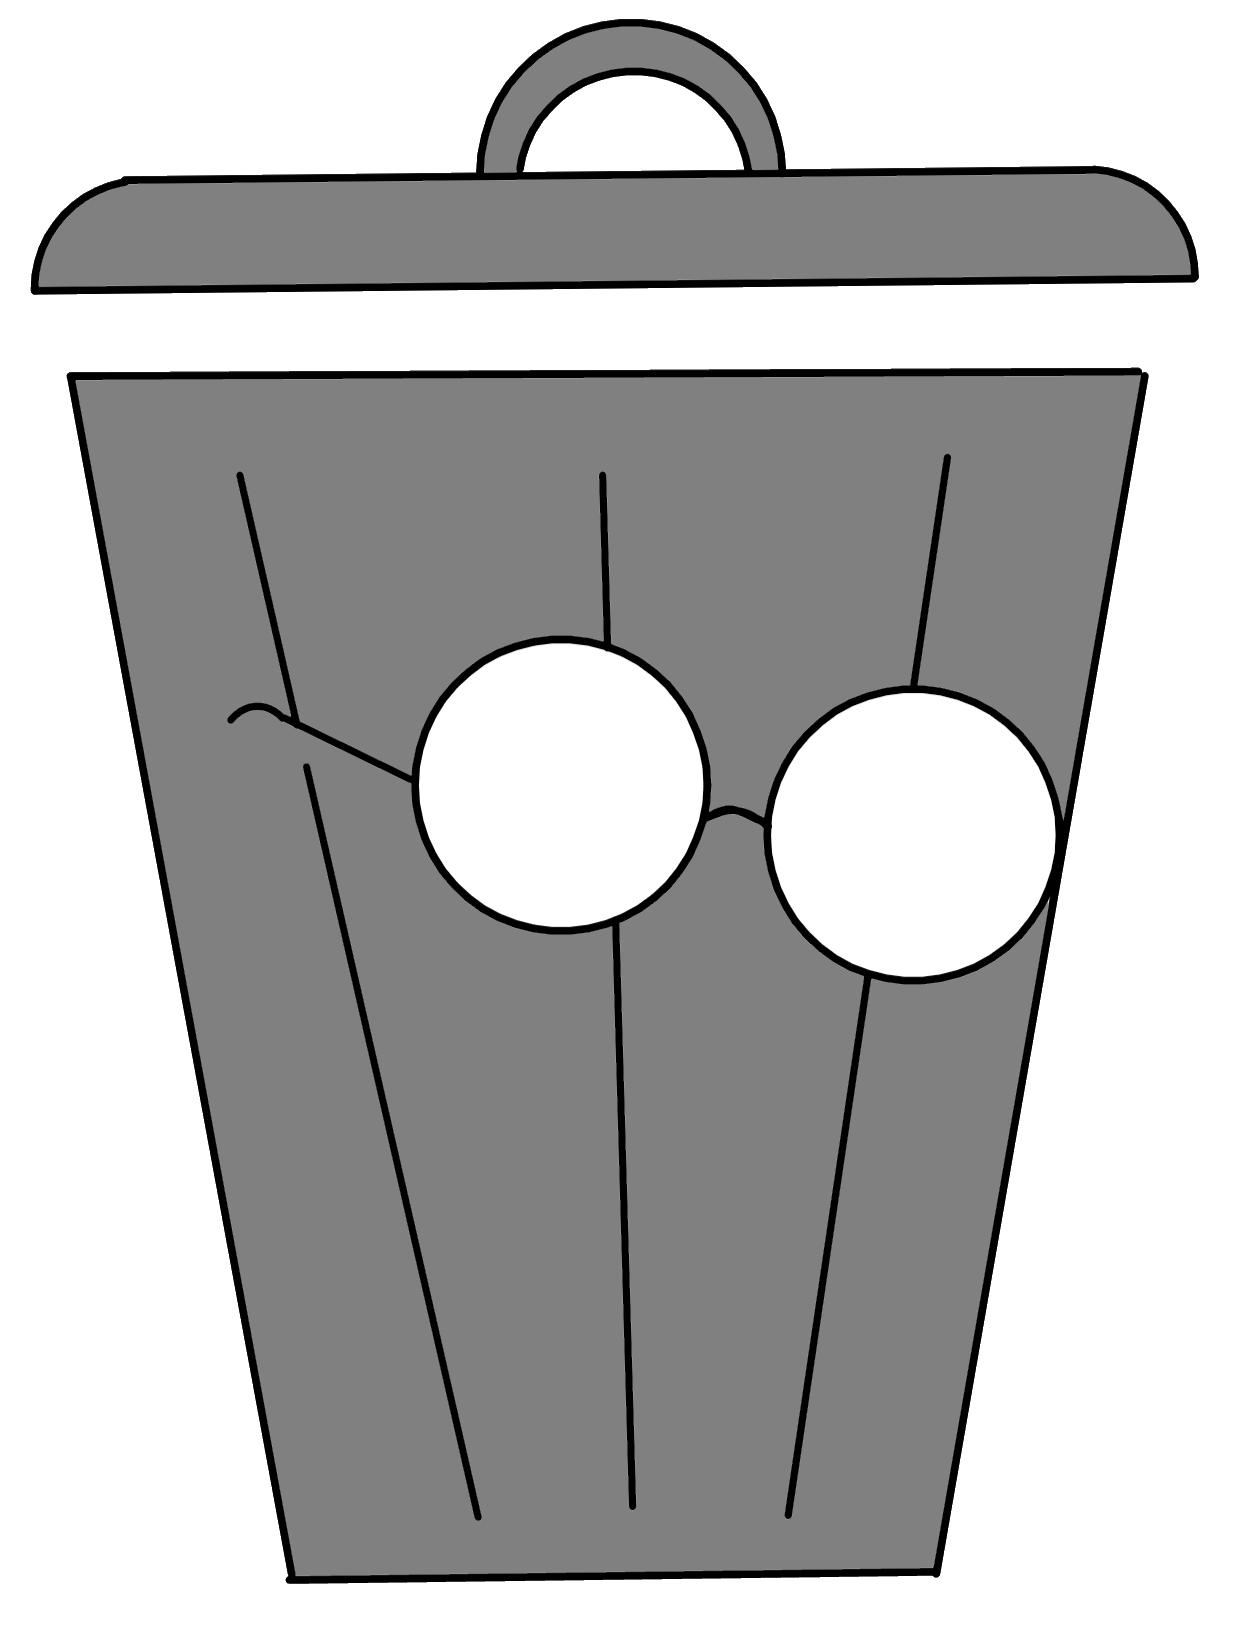
\includegraphics[width=6cm]{../graphical/logo_draft_color.png}}


\begin{document}
\maketitle

\null\vfill
\noindent
App Design Document\\ 
Mobile (App) Software Engineering\\
Technische Universität Wien\\
Version v1.0, März 2019
\newpage

\tableofcontents

% ______________________
% Kapitel Konzept
% ______________________
\chapter{Konzept}

\section{Geplanter Name der App}
Der gewählte Name der App ist Mr. Trash. Die Idee dahinter ist, dass der Name leicht zu merken ist und der User somit sich leicht merken kann "wen er fragen kann", wenn er/sie wissen will, "wohin mit dem Müll".

Weiters lässt sich dazu ein passendes Logo ableiten, dass schlicht ist und davon zeugt, dass die App die richtige sei, wenn es um Fragen im Themenbereich Müll geht.

\section{Kurzbeschreibung}
Mr.Trash ermöglicht es dem unerfahrenen Mülltrenner effizient den richtigen Ort, seinen Müll zu entsorgen, in seiner Nähe zu finden oder einfach um zu sehen ob es ok ist, diesen Müll im Haushaltsmüll zu entsorgen. Die App stellt sicher, dass nie wieder Müll falsch entsorgt wird und somit Umweltfreundlichkeit gewährleistet wird und der Nutzer möglichst wenig Zeit und Know-How benötigt um Müll richtig zu trennen.

Ganz nützlich ist die App für das Auffinden spezieller, zeitlich bedingt vorhandener, "Mobilen Problemstoffsammelstellen", die ebenfalls, samt verfügbaren Uhrzeiten, angezeigt werden.

Nach dem Starten der App, ist es dem User sofort möglich ein Produkt aus einer ausführlichen Liste (auch verfügbar unter wien.gv.at~\cite{muelltrennabc}) auszuwählen. Alternativ dazu kann er auch einfach die Suche im oberen Bereich zu nutzen um das gewünschte Produkt zu finden.

Sobald das zu entsorgende Produkt gefunden wurde, wird der User durch anklicken zu einem neuen Schirm geführt, wo ersichtlich ist, wie er sein Produkt entfernen kann. Wenn vorhanden, kann durch Klicken auf den rechten unteren Text in der Card den nahsten Ort (z.B. Mistplatz) auf einer Google Maps Karte angezeigt werden.

Alternativ dazu, kann der User auch den Floating Button rechts unten nutzen um einfach den nahsten korrekten Ort zur Müllentsorgung auf einer Karte angezeigt bekommen (unabhängig von Entsorgungsortart).

\section{Beschreibung der gewählten Datensätze}
\begin{itemize}
	\item Sämtliche Müll-Daten Wien \cite{alleMuell}
	\item Problemstoffsammelstelle Wien \cite{problemstoffsammelstellen}
	\item Altstoffsammelstelle Wien \cite{alstoffsammelstellen}
	\item Mistplätze Standorte Wien \cite{mistplaetze}
	\item Mobile Problemstoffsammelstelle Standorte Wien \cite{mobileProblemstoffsmst}
	\item Christbaumsammelstellen Wien \cite{christbaumsammelstellen}
	\item Mülltrenn ABC \cite{muelltrennabc}
\end{itemize}

% ______________________
% Kapitel Graphischer Entwurf
% ______________________

\chapter{Graphischer Entwurf} 

\section{High-Fidelity Mockup}
\begin{figure}[h]
\centering

\includegraphics[width=0.3\textwidth]{../graphical/test.jpg}
\caption{\label{fig:art1} Art example}
\end{figure}

\section{Product Icon}
\begin{figure}[h]
\centering
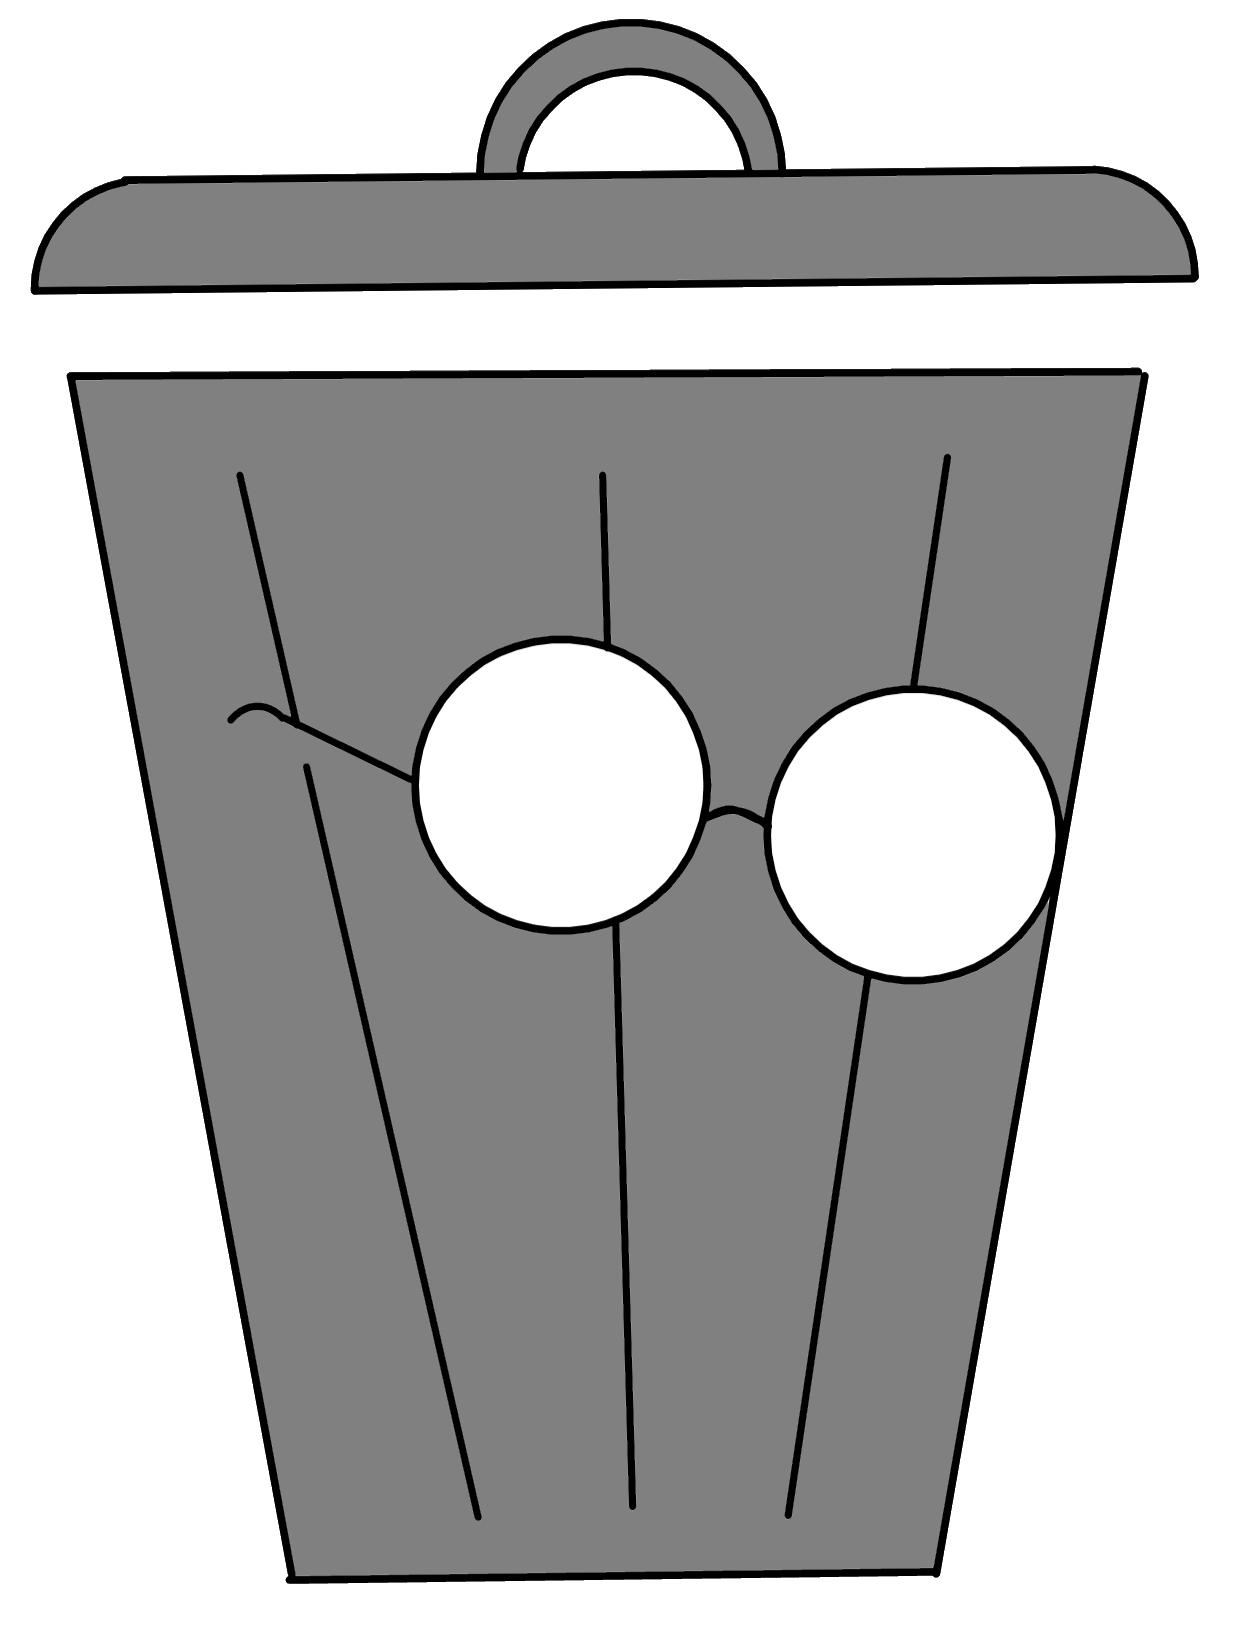
\includegraphics[width=0.3\textwidth]{../graphical/logo_draft_color.png}
\caption{\label{fig:logo} Mr. Trash Logo}
\end{figure}

\bibliographystyle{abbrv}
\bibliography{references}

\end{document}